\begin{frame}{Subgradient for non differentiable functions}
\begin{minipage}{0.5\textwidth}
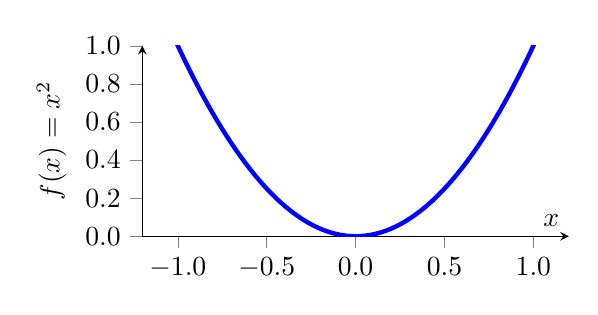
\begin{tikzpicture}
    \begin{axis}[
    	legend pos=north west,
        axis x line=middle,
        axis y line=left,
        x tick label style={/pgf/number format/fixed,
                            /pgf/number format/fixed zerofill,
                            /pgf/number format/precision=1},
        y tick label style={/pgf/number format/fixed,
                            /pgf/number format/fixed zerofill,
                            /pgf/number format/precision=1},
        %grid = major,
        width=7cm,
        height=4cm,
        grid style={dashed, gray!30},
        xmin=-1.2,     % start the diagram at this x-coordinate
        xmax= 1.2,    % end   the diagram at this x-coordinate
        ymin= 0,     % start the diagram at this y-coordinate
        ymax= 1,   % end   the diagram at this y-coordinate
        %axis background/.style={fill=white},
        xlabel={$x$},
        ylabel={$f(x)=x^2$},
        tick align=outside,
        enlargelimits=false]
      % plot the stirling-formulae
      \addplot[domain=-5:5, blue, ultra thick,samples=500] {x^2};
    \end{axis}
\end{tikzpicture}
\end{minipage}
\begin{minipage}{0.45\textwidth}
\begin{equation*}
\begin{aligned}
f(x) = x^2 \\
\nabla f(x) = 2x
\end{aligned}
\end{equation*}
\end{minipage}
\begin{minipage}{0.5\textwidth}
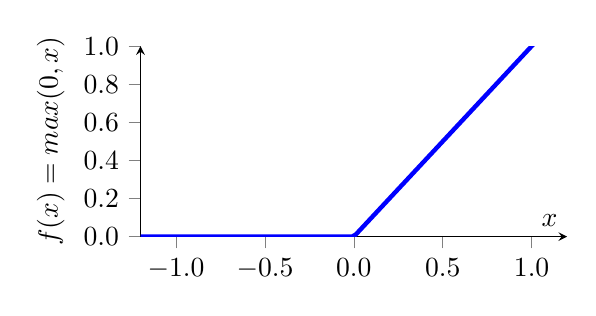
\begin{tikzpicture}
    \begin{axis}[
    	legend pos=north west,
        axis x line=middle,
        axis y line=left,
        x tick label style={/pgf/number format/fixed,
                            /pgf/number format/fixed zerofill,
                            /pgf/number format/precision=1},
        y tick label style={/pgf/number format/fixed,
                            /pgf/number format/fixed zerofill,
                            /pgf/number format/precision=1},
        %grid = major,
        width=7cm,
        height=4cm,
        grid style={dashed, gray!30},
        xmin=-1.2,     % start the diagram at this x-coordinate
        xmax= 1.2,    % end   the diagram at this x-coordinate
        ymin= 0,     % start the diagram at this y-coordinate
        ymax= 1,   % end   the diagram at this y-coordinate
        %axis background/.style={fill=white},
        xlabel={$x$},
        ylabel={$f(x)=max(0,x)$},
        tick align=outside,
        enlargelimits=false]
      % plot the stirling-formulae
      \addplot[domain=-5:5, blue, ultra thick,samples=500] {max(0, x)};
    \end{axis}
\end{tikzpicture}
\end{minipage}
\begin{minipage}{0.45\textwidth}
\begin{equation*}
\begin{aligned}
f(x) &= \max(0, x) \\
\nabla f(x) &= \begin{cases}
    1,& \text{if } x\geq 0\\
    0,& \text{if} x < 0
\end{cases}
\end{aligned}
\end{equation*}
\end{minipage}
\end{frame}